\begin{figure}
\centering
    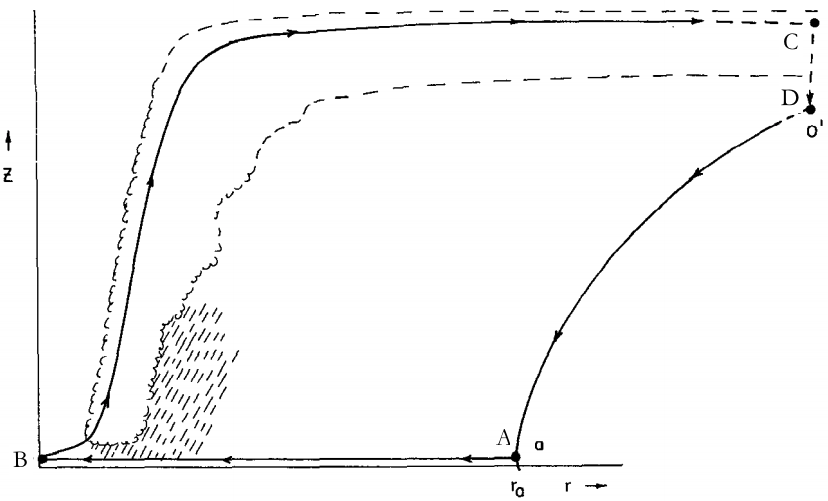
\includegraphics[width=\linewidth]{images/hurricane-carnot.png}\\
    \textit{Figure 1 from~\cite{emanuel1991theory}. }
    \caption{A Carnot cycle where air travels clockwise:
            A$\rightarrow$B travelling isothermally inwards to the eye-wall, extracting enthalpy
            from the sea, and gaining entropy through kinetic energy dissipation;
            B$\rightarrow$C moist adiabatically thrust up into the stratosphere
            at the eye-wall and out to the subsidence point;
            C$\rightarrow$D initial isothermal descent [some radiative loss];
            D$\rightarrow$A final moist adiabatic descent~\cite{emanuel2018progress}. }
            \label{fig:hurricane-carnot}

\end{figure}
